%%%% ijcai22-multiauthor.tex

\typeout{IJCAI--22 Multiple authors example}

% These are the instructions for authors for IJCAI-22.

\documentclass{article}
\pdfpagewidth=8.5in
\pdfpageheight=11in
% The file ijcai22.sty is NOT the same as previous years'
\usepackage{ijcai22}

% Use the postscript times font!
\usepackage{times}
\renewcommand*\ttdefault{txtt}
\usepackage{soul}
\usepackage{url}
\usepackage[hidelinks]{hyperref}
\usepackage[utf8]{inputenc}
\usepackage[small]{caption}
\usepackage{graphicx}
\usepackage{amsmath}
\usepackage{booktabs}
\usepackage{algorithm}
\usepackage{algorithmic}
\urlstyle{same}
\usepackage{xcolor}
\usepackage{multicol}
\usepackage{tikz}

\newcommand\todo[1]{\textcolor{red}{#1}}

% the following package is optional:
%\usepackage{latexsym}

\pdfinfo{
	/TemplateVersion (IJCAI.2022.0)
}


\title{A computational approach for variants of coloring planar graphs}

\author{
	Arne Claerhout$^1$\and
	Jorik Jooken$^1$\And
	Jan Goedgebeur$^1$\\
	\affiliations
	$^1$KU Leuven KULAK
	\emails
	arne.claerhout@student.kuleuven.be,
	jorik.jooken@kuleuven.be,
	jan.goedgebeur@kuleuven.be
}


\begin{document}
	
\maketitle

\begin{abstract}
	In this paper, we study the coloring of planar graphs for different variants of graph colorings. In particular the proper, odd, conflict-free and unique-maximum vertex colorings are examined. This paper proposes a backtracking algorithm to color planar graphs.
	
	The chromatic numbers of these coloring variants are also studied further. These are the minimum number of colors needed to color any planar graph.
	
	Not all chromatic numbers are known, therefore, conjectures exist. This algorithm can be used to disprove or substantiate these conjectures.
	
	The algorithm was constructed by applying optimizations to a naive algorithm. The final implementation is a fully optimized algorithm implemented in C.
	
	The proposed algorithm does not outperform alternatives, but is only less than $1.5$ times slower, for the proper coloring. No other programs exist for the other colorings. It also has the added benefit of easy expandability for other coloring variants.
	
	It was also found that the conjectures that haven't been disproven yet are correct for all planar triangulations with $20$ or less vertices. 
	
\end{abstract}

\section{Introduction}

Graph theory is a field of research in computer science that is older than the computer. Its conception dating back to the 18th century \cite{euler1741solutio}. 

A \textit{graph} $G = (V, E)$ is defined as a pair, containing a collection of vertices ($V$) and edges ($E$). Each edge is an unordered pair of unique vertices. A \textit{planar graph} is a variant of graphs such that a planar embedding is possible without edges crossing. Planar graphs and graphs will be used interchangeably. The \textit{class of planar graphs} $\mathcal{P}$ is defined as the set of all planar graphs. \textit{Planar triangulations}, a subset of planar graphs, are graphs with the maximum number of edges for some number of vertices, this means the addition of an edge would break the planarity of the graph.

The coloring of graphs is one of the most well-known fields in graph theory. A coloring of a graph is a function assigning each vertex a color $1, \dots, k$. The most famous of these colorings is the proper coloring. This states that two adjacent vertices -- vertices sharing an edge -- never share the same color. 

The chromatic number $\chi(G)$ of a graph $G$ is the minimum number of colors needed to color the graph. A generalization of this is the chromatic number $\chi(\mathcal{P})$ for the class of planar graphs, which is the minimum number of needed colors to color \textit{any} planar graph. For the proper coloring, it was proven that four colors always suffice \cite{appel1976every}. This was a special result, as this was the first proof verified using a computer program.

Coloring of graphs has various applications, with uses including: the assignment of frequencies to radio stations, the coloring of maps, scheduling and more.

There exist many variants of graph colorings. One such variant is an \textit{odd coloring}, which was recently introduced by Petruševski and Škrekovski \cite{PETRUSEVSKI2022385} in $2022$. A proper coloring of a graph is said to be odd if for each vertex $v \in V$ there exists a color occurring an odd amount of times in the neighborhood of that vertex $N(v)$. The \textit{odd chromatic number} $\chi_{\mathrm{O}}(\mathcal{P})$ is the minimal number of colors needed to color any graph with an odd coloring.

Other variants include the conflict-free and unique-maximum colorings. 

The \textit{conflict-free coloring}, introduced in 2003 by Even, Lotker, Ron, and Smorodinsky \cite{even2003conflict}, is a coloring such that every vertex has at least one unique color in its neighborhood. This is useful because of applications in wireless networks and more \cite{smorodinsky2013conflict}.

Now consider a \textit{proper conflict-free coloring} with respect to open- or closed neighborhoods -- a conflict-free coloring with an added proper constraint. The conflict-free property is tested on the open- or closed neighborhood of vertices. 
An open neighborhood of a vertex $v$ is defined as $N(v) = \{w | (v, w) \in E\}$. This does therefore not include the vertex $v$ itself. A closed neighborhood of a vertex $v$ is $N[v] = N(v) \cup \{v\}$, the open neighborhood of $v$, including the vertex itself. 
Both colorings have \textit{chromatic numbers} $\chi_{\mathrm{pCFo}}(\mathcal{P})$ and $\chi_{\mathrm{pCFc}}(\mathcal{P})$ respectively, with the $o$ and $c$ signaling open- or closed neighborhoods.


Similarly, an \textit{improper conflict-free coloring} with respect to open- or closed neighborhoods can be defined. These are the same colorings, without the proper constraint. Again, \textit{chromatic numbers} $\chi_{\mathrm{iCFo}}(\mathcal{P})$ and $\chi_{\mathrm{iCFc}}(\mathcal{P})$ respectively can be defined for both.

\textit{Unique-maximum colorings} stem from ordered colorings \cite{KATCHALSKI1995141}, and were studied further in the context of open- and closed neighborhoods by Fabrici, Lužar, Rindošová and Soták \cite{fabrici2023proper}. This is a coloring where the maximum color appearing in the neighborhood of a vertex appears exactly once in the neighborhood of that vertex.

Using the same splitting as the conflict-free coloring, four versions of this coloring can be defined. A proper unique-maximum coloring with respect to open- or closed neighborhoods, and an improper unique-maximum coloring with respect to open- or closed neighborhoods. Each respectively having their own \textit{chromatic number} for the class of planar graphs: $\chi_{\mathrm{pUMo}}(\mathcal{P})$, $\chi_{\mathrm{pUMc}}(\mathcal{P})$, $\chi_{\mathrm{iUMo}}(\mathcal{P})$ and $\chi_{\mathrm{iUMc}}(\mathcal{P})$.

\subsection{Known bounds}

Not all chromatic numbers of these colorings are known. For most, only bounds exist, where some upper bound always suffices to color all graphs, while the lower bound is derived from a graph with the highest \textit{found} chromatic number. 

As the unique color for each vertex $v$ in the $\mathrm{pCFc}$-coloring can always be the color of $v$ itself, this coloring is exactly equal to the proper coloring. Therefore, $\chi_{\mathrm{pCFc}}(\mathcal{P})$ is, just like the chromatic number of the proper coloring, equal to $4$.

The bounds for all colorings are as follows:


\begin{itemize}
	\item The odd coloring:
	\begin{itemize}
		\item $5 \leq \chi_{\mathrm{O}}(\mathcal{P}) \leq 8$ (\textit{proven by \cite{petr2023odd} for upper bound, lower bound is $\mathit{C_5}$})
	\end{itemize}
	
	\item the conflict-free colorings:
	\begin{itemize}
		\item $6 \leq \chi_{\mathrm{pCFo}}(\mathcal{P}) \leq 8$ (\textit{proven by \cite{fabrici2023proper}})
		\item $\chi_{\mathrm{pCFc}}(\mathcal{P}) = 4$
		\item $4 \le \chi_{\mathrm{iCFo}}(\mathcal{P}) \le 5$ (\textit{proven by \cite{abel2018conflict} for lower bound and \cite{huang2020short} for upper bound})
		\item $\chi_{\mathrm{iCFc}}(\mathcal{P}) = 4$ (\textit{proven by \cite{Malik2023thesis}})
	\end{itemize}
	
	\item The unique-maximum colorings (all \textit{proven by \cite{fabrici2023proper}}):
	\begin{itemize}
		\item $6 \leq \chi_{\mathrm{pUMo}}(\mathcal{P}) \leq 10$
		\item $6 \leq \chi_{\mathrm{pUMc}}(\mathcal{P}) \leq 8$
		\item $5 \le \chi_{\mathrm{iUMo}}(\mathcal{P}) \le 10$
		\item $4 \le \chi_{\mathrm{iUMc}}(\mathcal{P}) \le 6$
	\end{itemize}
\end{itemize}



\subsection{Conjectures}
\label{sect:Conjectures}

As most of the chromatic numbers are not known. Some authors started formulating conjectures on this problem.

Petruševski and Škrekovski, the originators of the odd coloring, conjectured $\chi_{\mathrm{O}}(\mathcal{P}) = 5$. Other conjectures introduced by Fabrici, Lužar, Rindošová and Soták \cite{fabrici2023proper} include:

\begin{minipage}{0.45\textwidth}
	\raggedcolumns
	\begin{multicols}{2}
		\begin{itemize}
			\item $\chi_{\mathrm{pUMo}}(\mathcal{P}) \leq 7$
			\item $\chi_{\mathrm{pUMc}}(\mathcal{P}) = 6$
			\item $\chi_{\mathrm{iUMo}}(\mathcal{P}) = 5$
			\item $\chi_{\mathrm{iUMc}}(\mathcal{P}) = 4$
			\item $\chi_{\mathrm{pCFo}}(\mathcal{P}) = 6$
			\item $\chi_{\mathrm{iCFo}}(\mathcal{P}) = 4$
			\item $\chi_{\mathrm{iCFc}}(\mathcal{P}) = 3$
		\end{itemize}
	\end{multicols}
\end{minipage}
\vspace{0.4cm}

Since then, the conjecture for the chromatic number of the $\mathrm{iCFc}$-coloring has been disproven.


\subsection{Research Problem}

In this paper, two research questions are considered:

\begin{itemize}
	\item \textbf{Can we design an algorithm for coloring planar graphs, faster than or just as fast as the existing coloring algorithms, that is also easily expandable to new coloring variants?}
	\item \textbf{In what way is this algorithm useful in helping to prove or disprove conjectures surrounding these coloring variants?}
\end{itemize}

The focus is mostly laid on the designing of the algorithm. Further results are also discussed.

The structure of this paper is as follows. First, the algorithm developed is discussed in Section \ref{sec:alg} by examining the the pseudo-code. Afterwards, the implementation of said algorithm is discussed in Section \ref{sec:implementation}. Here, all notable optimizations applied are studied further. Then, the results of this paper are discussed further in Section \ref{sec:results}. Thereafter, the threats to validity are discussed in Section \ref{sec:threats}, ending with the conclusion in Section \ref{sec:conclusion}.


\section{Algorithm}
\label{sec:alg}

In this section the developed algorithm is discussed. A backtracking algorithm was used, coloring the vertices one-by-one and pruning where possible. The pseudo-code is found in Algorithms \ref{alg:search}, \ref{alg:check}, \ref{alg:updateN} and \ref{alg:special}. 


Starting with Algorithm \ref{alg:search}, this is the `overseer' of the algorithm. Only choosing a maximum color for the graph and letting the recursive algorithm check if the coloring is possible for that maximum.
This is also reflected in the pseudo-code. 

Before checking the maximum color, the available colors of the vertices are reset to reflect the maximum color (\textit{e.g., if the maximum color is 3, the available colors are ${1, 2 \text{ and } 3}$}).

Algorithm \ref{alg:check} is the main checking algorithm. It checks whether the given graph $G$ is able to be colored given a maximum color $max\_c$. This happens in multiple steps, starting with the base case. If all vertices are colored, a valid coloring is reached and the previous recursion step is notified of this. 

Otherwise, it loops over all available colors of the given vertex, where it checks if that available color is one higher or less than the current maximum color in the graph. This optimization is further discussed in Section \ref{sec:optim}.

Next, the $vertex$ is colored in the available color $c$, and all neighbors of that $vertex$ are updated using the \texttt{update\_neighbors} function. This will essentially update the available colors of all neighbors and those neighbors' neighbors, and check if the coloring is still possible. If not, the progress made this recursion step is reset, and the next available color is tried. If the coloring is \textit{still} possible, the next recursion step is called with a new $index$ and $depth$. 

The \texttt{update\_neighbors} function is therefore the function checking the correctness of the coloring. If the coloring isn't valid, the graph goes back a recursion step, essentially backtracking. All checks are done while the algorithm is coloring, this means no check has to happen in the base case.

After trying all available colors without results, the vertex color is reset and the previous recursion step is notified of failure.

The $depth$ variable is used in the \texttt{add\_colors\_back} function. All of the changes in the entire algorithm, meaning all updates for all vertices and all recursion steps, are kept track of. The depth is used to log changes and restoring them.

Lastly, Algorithm \ref{alg:updateN} updates neighbors of a given $vertex$ for a given color $c$, the color assigned to $vertex$. Here, the available colors of all uncolored neighbors of $vertex$ are updated when the coloring $K$ is proper (\textit{e.g., $\mathrm{pUMo}$, odd, $\dots$}). If this leads to a neighbor having no available colors, the coloring isn't valid and the pruning starts.

Otherwise, the neighborhood of the neighbors are checked. If these are fully colored (because the last vertex $vertex$ was colored in just now), the correctness is checked for coloring $K$, again, if this isn't valid, prune, otherwise, keep going. 

Finally, if the neighborhood of the neighbor still has one vertex left to color, the available colors for this vertex are updated. This is achievable for most colorings, except the proper coloring. A concrete example is worked out in Algorithm \ref{alg:special} for the odd coloring. Here, all other vertices' colors are used to check compatibility with the available colors of the uncolored vertex $u$. In this case, the odd constraint is checked, if only one color appears an odd amount of times, $u$ can not have this color.
For the other colorings, similar rules are applied to update the vertex $u$.

% Search
\begin{algorithm}[tb]
	\caption{\texttt{search\_chromatic\_number}}
	\label{alg:search}
	\textbf{Parameters}: The coloring $K$
	
	\textbf{Output}: Chromatic number
	\begin{algorithmic}[1]
		\STATE $\mathcal{G} \gets \text{graphs generated by \textit{plantri}}$
		\FOR{\texttt{$G \in \mathcal{G}$}}
		\FOR{\text{$max\_c$ $ \le $ $10$}}
		\STATE \texttt{set\_max\_color\_for\_vertices}($G$)
		\IF{\texttt{can\_color\_with\_max\_c}($G, K, 0, max\_c, 0, 0$)} 
		
		\RETURN $max\_c$
		\ENDIF
		\ENDFOR
		\ENDFOR
	\end{algorithmic}
\end{algorithm}

% Check
\begin{algorithm}[tb]
	\caption{\texttt{can\_color\_with\_max\_c}}
	\label{alg:check}
	\textbf{Parameters}: The graph $G$, coloring $K$, max. color in graph $max\_c\_in\_g$, max. color $max\_c$, $index$ and $depth$\\
	\textbf{Output}: Coloring achieved
	\begin{algorithmic}[1]
		\IF{All vertices colored}
		\RETURN true
		\ENDIF
		\STATE $vertex \gets G.vertices$[$index$]
		\FOR{available color $c$ of $vertex$}
		\IF{$\neg$\texttt{is\_UM}($K$) and $c > max\_c\_in\_g + 1$}
		
		\STATE continue
		\ENDIF
		
		\STATE $vertex.color \gets c$
		\STATE $new\_max\_c\_in\_g \gets \max(max\_c\_in\_g, c + 1)$
		
		\IF{\texttt{update\_neighbors}($G, K, vertex, c, depth$)}
		
		\STATE \texttt{add\_colors\_back}($G, depth$)
		\STATE continue
		\ENDIF
		\IF{\texttt{can\_color\_with\_max\_c}($G, K, new\_max\_c\_in\_g,$ $max\_c, $ \texttt{getBestIndex}()$, depth + 1$)}
		
		\RETURN true
		\ENDIF
		\STATE \texttt{add\_colors\_back}($G, depth$)
		
		\ENDFOR
		
		\STATE $vertex.color \gets 0$
		\RETURN false
	\end{algorithmic}
\end{algorithm}

% update neighbors
\begin{algorithm}[tb]
	\caption{\texttt{update\_neighbors}}
	\label{alg:updateN}
	\textbf{Parameters}: The graph $G$, coloring $K$, vertex $v$ to update, color $c$ of $v$ and $depth$ of algorithm \\
	\textbf{Output}: Coloring impossible
	\begin{algorithmic}[1]
		\FOR{$n \in $ $vertex.neighbors$}
		
		\IF{\texttt{is\_proper}(coloring $K$) and $n.color = 0$}
		
		\IF{\texttt{remove\_available\_c}($G, n, c, depth$)}
		
		\RETURN true 
		\ENDIF
		\ENDIF
		
		\IF{$n.neighbors$ is fully colored and $\neg$\texttt{is\_correctly\_colored}($K, n$)}
		
		\RETURN True
		\ELSIF{$n.neighbors$ contains only \textbf{one} uncolored vertex $u$}
		\IF{\texttt{handle\_special\_case}($K, u, n.neighbors,$ $ depth$)}
		
		\RETURN true
		
		\ENDIF
		\ENDIF
		\ENDFOR
		\RETURN false
	\end{algorithmic}
\end{algorithm}

% handler
\begin{algorithm}[tb]
	\caption{\texttt{handle\_special\_case\_odd}}
	\label{alg:special}
	\textbf{Parameters}: The coloring $K = $ odd, vertex to update $u$, $neighbors$ and $depth$ \\
	\textbf{Output}: Coloring impossible
	\begin{algorithmic}[1]
		\STATE $colors\_odd = \{\}$
		\FOR{$neighbor \in neighbors \setminus \{u\}$}
		
		\IF{$neighbor.color \in colors\_odd$}
		
		\STATE $colors\_odd = colors\_odd \setminus \{neighbor.color\}$
		
		\ELSE 
		
		\STATE $colors\_odd = colors\_odd \cup \{neighbor.color\}$
		\ENDIF
		
		\ENDFOR
		
		\IF{$\left| colors\_odd \right| = 1$}
		
		\RETURN \texttt{remove\_available\_c}($G, u, colors\_odd, depth$)
		\ENDIF
		\RETURN false
	\end{algorithmic}
\end{algorithm}

It is clear that the algorithm can color in graphs, and find the chromatic number of that graph for a given coloring, since all possible colorings are tried and checked except those that can be pruned.

\section{Implementation}
\label{sec:implementation}

The algorithm was developed by working out the code for an efficient backtracking algorithm. This was done in multiple stages. First, this was developed in Java to test out different data structures and techniques, and to optimize the algorithm. Afterwards, the optimal implementation found in Java, reflecting the algorithm discussed, was then ported over to C. All versions of the implementation and other help scripts are open-source\footnote{The \href{https://github.com/ArneClaerhout/color_planar_graphs}{GitHub repository} containing the algorithm.}.

The implementation uses \textit{plantri}, a fast generator of planar graphs developed by Brinkmann and McKay \cite{brinkmann2007fast}. \textit{Plantri} is a tool that is able to generate all planar graphs for a given number of vertices. This allows the program to easily generate and color graphs at once when some number of vertices is given. 

\subsection{Optimizations}
\label{sec:optim}

Here, the most important optimizations influencing the execution time are explained. For most, the impact on the speed is measured, to justify the usage of these optimizations. All of the comparisons are measured at the relevant stage of development, so that the code could be kept as clean as possible. A slower ``optimization'' was therefore never implemented again in newer implementations.

For all experiments, a laptop with an intel i7 CPU was used, using windows as the OS and WSL to execute the program. Each experiment was performed three times to counteract noise on the data.
All figures used in this section are using these results. Since there are $9$ unique colorings to consider, the cumulative needed time for all colorings is used as the performance measure.

\subsubsection{Available colors}

The first optimization used, is keeping track of the available colors per vertex. This allows the algorithm to prune early whenever a vertex has no possible colors left. Comparing this to a naive algorithm, yields expected results. Without any other optimizations, this is only applicable for proper colorings (\textit{e.g., $\mathrm{pUMo}$, proper}). Therefore, there is no effect on improper colorings. 

\subsubsection{Permutations}

As illustrated in Algorithm \ref{alg:check}, permutations of already tried colorings of the graph are prohibited, except for unique-maximum colorings. For non-unique-maximum colorings, swapping colors (\textit{e.g., changing all vertices colored $2$ to color $3$ and vice versa}) still yields a valid coloring. This dramatically cuts down the search space. 

This isn't the case for a unique-maximum coloring because swapping two colors doesn't always yield a valid coloring (\textit{e.g., swapping the maximum color with a color occurring twice in a neighborhood}). Therefore, all possible colorings should get checked for the unique-maximum colorings. 

\subsubsection{Bit-sets}
\label{sec:bitset}

Another optimization used, which is not visible in the pseudo-code of the algorithm, is the use of bit-sets. Instead of each vertex having a list of all neighboring vertices as objects, only the indices of the neighbors are stored. This is done in a binary number. If a vertex has a neighbor with index $i$, the neighbors bit-set has a $1$ at index $i$, starting from the least significant bit. 

This optimization allows for easier comparison between neighborhoods. Checking if some vertex is present in a neighborhood becomes simple, it happens in constant time instead of worst-case linear time. 

This optimization, together with the available colors optimization make up the optimized implementation found in Figure \ref{fig:general}. Compared to the naive implementation, a version not having these optimizations, these optimizations clearly have effect on the computation time and are therefore used.

\begin{figure}
	\centering
	
\includegraphics[width=0.45\textwidth]{figures/General_comparison.pdf}
	\caption{A comparison between different versions of the algorithm, tested on all planar triangulations for a given number of vertices. The naive algorithm is the simplest algorithm described in Algorithm \ref{alg:naive}. Optimized is the implementation that has implemented the available colors, permutations and bit-sets optimizations. The second order implementation has also implemented the updating of neighbors' neighbors. Lastly, the final and multithreaded implementations are the final C implementation and its multithreaded version using 10 processes respectively. Each implementation performs better than the last.}\label{fig:general}
\end{figure}


\subsubsection{Data structures}

For the implementation of the algorithm, multiple data structures for monitoring vertices were tested.
These include a simple list of vertices, a priority queue and a bit-set implementation. The speed of these data structures are tested against each other.

These structures are all considered because of some strengths these seemingly have. The list of vertices is very simple, and could therefore work well. The priority queue sorts the vertices by the amount of available colors (from low to high), and therefore has easy look-up for the best vertex to color in. And lastly, the bit-set data structure, implemented using a list of bit-sets, where each index of the list denotes a number of available colors. The bit-sets then indicate if a vertex either has or doesn't have a certain amount of available colors.

The comparison between datastructures is found in Figure \ref{fig:datastruct}. It is clear the priority queue method performs the worst. This is because updating the number of available colors requires a completely new entry in the queue, which has too much overhead. Both the bit-set and standard list implementation perform almost equally well in the figure. Since the scale of the y-axis in the figure is logarithmic, the difference is still substantial.
Going forward, the simple list datastructure is used.

\begin{figure}
	\centering
	
\includegraphics[width=0.45\textwidth]{figures/Datastructures_comparison.pdf}
	\caption{A comparison between the discussed datastructures. The simple list structure performs the best.}\label{fig:datastruct}
\end{figure}

\subsubsection{Index}

In total, five different \texttt{get\_best\_index}-techniques were tested out. These techniques ranged from simply finding the vertex with the least amount of available colors, to finding the vertex with the highest degree. Some methods were adapted from results found by Aslan and Baykan \cite{aslan2016performance}. Of these $5$, the best-performing and simplest methods are compared.

These include the two previously-mentioned methods, respectively called Standard and Welsh Powell (WP), are compared against Standard\_WP: a combination of the two techniques, using the standard technique with a degree tiebreaker. 

Other methods mentioned by Aslan and Baykan, such as DSATUR and First Fit either had overhead in registering extra data specifically for the technique, or were too simple and therefore performed badly in the original paper. Thus, these are not considered.

Figure \ref{fig:index} shows the comparison of the three discussed techniques. Here, there is no doubt that the standard least amount of available colors performs best. It does look like both curves grow as fast for the number of vertices, but the growth phase of the standard technique starts later. Therefore, this index-choosing technique is used from here on out. 

\begin{figure}
	\centering
	
\includegraphics[width=0.45\textwidth]{figures/Index_comparison.pdf}
	\caption{The choosing of next vertex indices is compared for $3$ methods. WP and Standard\_WP perform almost equal. The standard method grows the slowest.}\label{fig:index}
\end{figure}


\subsubsection{Second order optimization}
\label{sec:secondorder}

Instead of only updating the available colors of vertices' neighbors, those of the neighbors' neighbors can also change when coloring a vertex. Here, this is only done when there is only one uncolored vertex left in the neighborhood of the neighbor. One of those rules is displayed in Algorithm \ref{alg:special} for the odd coloring. As mentioned before, the other colorings also have similar rules.

The rule for the unique-maximum coloring checks the number of times the maximum color occurs, if this is only once, prohibit the use of that color, otherwise, the uncolored vertex needs an even higher color to create a new maximum color.

The conflict-free rule checks whether any colors occur once, if not, the uncolored vertex should get a unique color. Otherwise, if there is only one color occurring once, this color should get avoided, if there are multiple, nothing happens. 

The effect of using these second-order optimizations is visible in Figure \ref{fig:general}. This optimization clearly makes the algorithm perform better. It even results in a slower growth of needed time.

\subsubsection{Parallelization}

A simple but effective optimization to apply is the use of parallelization. By using the already defined $RES/MOD$ option in \textit{plantri}, an option to split up the generated graphs into disjoint sets, the coloring of the graphs is easily done using multiprocessing. A procedure where a new process is created for each of the independent sets generated. This allows for a significant speedup dependent on the architecture of the system used (\textit{i.e., number of cores}). Because now more of the cores of the CPU are used, instead of only one.
All outputs are then generated in different output files and combined at finish time.

A comparison between the normal and multiprocessed implementations is shown in Figure \ref{fig:general}. As expected, for less graphs, splitting up all graphs, and combining the results will take longer than only coloring the graphs. After planar triangulations with $12$ vertices, the speedup of using multiprocessing does become apparent. 

\subsubsection{Porting to C}

The last optimization is the moving of the code from Java to C, a low-level programming language. The difference between the two languages is in the extra overhead found in Java. Java uses features like a garbage collector to monitor memory usage. C does not, which allows it to process graphs faster, but it does call for a more careful approach.

Only the best-performing datastructures and optimizations are added in C. These will therefore not be compared again in C.

Figure \ref{fig:general} shows a comparison between the Java second order implementation and the Final C implementation. The final version does have extra smaller optimizations, but even comparing both on almost the exact same implementation still favours C.


\subsection{Correctness}
\label{sec:correctness}

The correctness of the implemented algorithm is never guaranteed. This is different for very simple versions of the algorithm. By comparing a naive implementation to the final implementation in C, discrepancies in coloring results can get found and resolved. 

% naive
\begin{algorithm}[tb]
	\caption{\texttt{can\_color\_with\_max\_c\_naive}}
	\label{alg:naive}
	\textbf{Parameters}: The graph $G$, coloring $K$, max. color $max\_c$ and $index$ \\
	\textbf{Output}: Coloring achieved
	\begin{algorithmic}[1]
		\IF{$index \ge G.nb\_vertices$}
		
		\RETURN \texttt{is\_correctly\_colored}($G, K$)
		\ENDIF
		
		\FOR{$c \le max\_c$}
		
		\STATE $G.vertices$[$index$]$.color \gets c$
		
		\IF{\texttt{can\_color\_with\_max\_c\_naive}($G, K, max\_c, index$)}
		
		\RETURN true
		
		\ENDIF
		
		\ENDFOR
		
		\RETURN false
	\end{algorithmic}
\end{algorithm}

The naive algorithm is displayed in Algorithm \ref{alg:naive}. The code reflects the pseudo-code almost one-to-one. From this, it is clear that the naive implementation works by testing every possible coloring given a maximum color. This implementation can therefore be considered correct.

All planar triangulations with number of vertices $4 \le v \le 12$ were tested for all colorings. 
For the proper coloring, an extra tool called \textit{nauty} developed by McKay and Piperno, is used \cite{mckay2014practical}. This tool can find the chromatic numbers for any graph very efficiently. Therefore, more planar triangulations were tested, those with number of vertices $4 \le v \le 20$.
The improper colorings (\textit{e.g., $\mathrm{iUMc}$}) use less colors overall, therefore these were tested to a maximum of $14$ vertices.

All tests found that the final implementation works correctly.

\section{Results}
\label{sec:results}

Now that the researched problem and the developed algorithm have been discussed, the research questions are revisited. 

The only existing coloring variant for which any algorithms exist, is the proper coloring. As mentioned before, this includes tools like \textit{nauty}. No open-source coloring tool for the other colorings exists. This means a comparison for efficiency for all coloring variants isn't possible.

Comparing \textit{nauty}'s coloring option against the developed algorithm has expected results. As seen in Table \ref{tab:nauty}, \textit{nauty} is faster in coloring all planar triangulations with some number of vertices. It can be noted that the program developed here is still performing well. Only less than $1.5$ times slower than \textit{nauty}. For higher number of vertices, the ratio between the two is getting smaller, indicating this program may be better for graphs with a high number of vertices.


\begin{table}
	\centering
	\begin{tabular}{r|ll|r} 
		\hline
		Number of vertices & This program ($s$) & \textit{Nauty} ($s$) & Ratio \\
		\hline
		$10$ & $0.013$ & $0.003$ & $4.3$ \\ 
		$11$ & $0.014$ & $0.004$ & $3.5$ \\
		$12$ & $0.020$ & $0.008$ & $2.5$ \\
		$13$ & $0.064$ & $0.039$ & $1.64$ \\
		$14$ & $0.39$ & $0.25$ & $1.56$ \\
		$15$ & $2.9$ & $1.9$ & $1.54$ \\
		$16$ & $22$ & $15$ & $1.49$ \\
		$17$ & $177$ & $121$ & $1.46$ \\
		$18$ & $1.4 \times 10^{3}$ & $1.0 \times 10^{3}$ & $1.41$
	\end{tabular}
	\caption{A comparison between the program developed in this paper and \textit{nauty}. Compared for all planar triangulations with a given number of vertices. \textit{Nauty} outperforms this program for all number of vertices. The ratio between the two tools goes down for more number of vertices.}\label{tab:nauty}
\end{table}


\textit{Nauty} is specifically designed for the coloring with the proper coloring. The other colorings discussed here are not supported. These would also require the addition of completely new functions, and a lot of code duplication; or a complete rework of the algorithm. Therefore, \textit{nauty} can not be easily expanded to new colorings, such as those discussed here, whereas this is possible for the developed algorithm. All coloring-dependent methods can be easily expanded without much added work. 
Additionally, \textit{nauty} does not automatically support the use of multiprocessing, while this is supported for our implementation. 

The other colorings are not comparable to other tools. Therefore, profiling the speed or efficiency of the algorithm is hard. But it does compare quite well to \textit{nauty}, and is also very expandable, which does mean it is efficient in that sense.


The second research question concerned the use of the algorithm for . This is an exhaustive algorithm, checking all possible graphs. Therefore, by processing all planar graphs for a given number of vertices, conjectures can be disproven or substantiated.

Here, all planar triangulations -- graphs with the highest possible number of edges and therefore graphs with a higher average chromatic number -- with $n$ vertices were checked ($4 \le v \le 20$). It was found that these graphs all conform to the current conjectures on chromatic numbers for all colorings.

The program can also assist in disproving the conjectures. An option is provided that will check all possible colorings of a given graph. This allows the user to assert if a graph has a certain property, helping in the search for gadgets -- graphs which help in the disproving or proving of some theorem or conjecture. 

The unique-maximum colorings have a property useful in the finding of gadgets, which the program can search for. As visible in Figure \ref{fig:graph}, there exist graphs with vertices that always have a certain color. These are great examples of gadgets, findable by the program. This is only applicable to these colorings, because as said before, permutations of other colorings still lead to a valid coloring. So no vertex can always have the same color.

\begin{figure}
	\begin{center}
		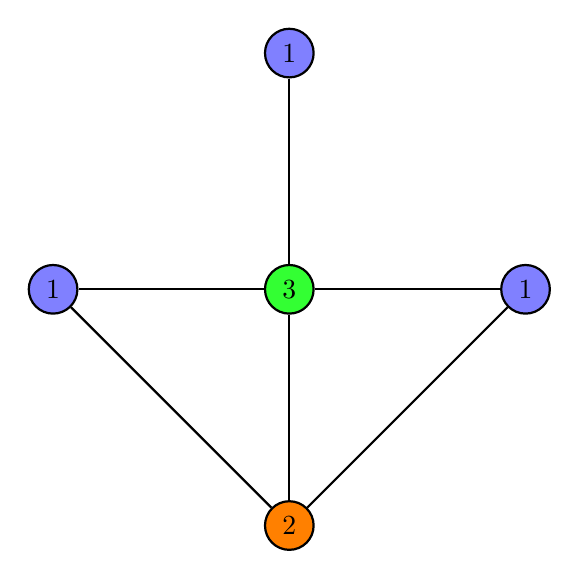
\begin{tikzpicture}[
			% Define the style for the nodes
			every node/.style={circle, draw, thick, minimum size=5mm}
			]
			
			\node (v1) at (0, 0) [fill=orange]  {2};
			\node (v2) at (0, 6) [fill=blue!50] {1};
			\node (v3) at (-3, 3) [fill=blue!50]{1};
			\node (v4) at (3, 3) [fill=blue!50]{1};
			\node (v5) at (0, 3) [fill=green!80]{3};
			
			\draw[thick] (v1) -- (v3);
			\draw[thick] (v1) -- (v4);
			
			\draw[thick] (v5) -- (v1);
			\draw[thick] (v5) -- (v2);
			\draw[thick] (v5) -- (v3);
			\draw[thick] (v5) -- (v4);
			
		\end{tikzpicture}
	\end{center}
	\caption{A colored graph for the $\mathrm{pUMo}$ coloring, where each vertex with color $1$ can only have that color. Giving it any other color would result in an invalid coloring.}\label{fig:graph}
\end{figure}


\section{Threats to validity}
\label{sec:threats}

As explained in Section \ref{sec:correctness}, the correctness of the implementation is never guaranteed. Furthermore, the comparison between implementations also doesn't guarantee correctness for graphs that were never tested, such as graphs with a high number of vertices. 
There is still a possibility that even the naive implementation isn't implemented correctly. However, this is unlikely because of the perfect reflection between implementation and algorithm. Still, the \texttt{is\_correctly\_colored}-check, seen in Algorithm \ref{alg:naive}, could function incorrectly.

The output of the proper coloring was tested against \textit{nauty}. There is no guarantee of the correctness of \textit{nauty}'s implementation.

All optimization experiments were performed on one specific machine, other computer architectures could yield a different outcome. 
Additionally, comparison of implementation decisions -- the optimizations presented -- are only tested at one implementation stage (\textit{e.g., naive implementation, post-bit-set implementation}), all tested in Java, and not at each stage of implementation. This could mean that some optimizations applied to the final program may result in different observations. For example, results of optimizations could differ when implemented in C.

\section{Conclusion}
\label{sec:conclusion}

In conclusion, this paper discussed a computational approach for the coloring of graphs. This is done for different variants of vertex colorings: namely the proper, odd, conflict-free and unique-maximum colorings. 

A backtracking algorithm for coloring planar graphs with these coloring variants is discussed. Firstly, the algorithm was developed in Java, to then be ported over to C for efficiency. In Java, multiple optimizations were tested out and implemented. Different data structures were considered, a simple list performing the best. Additionally, other optimizations such as the usage of bit-sets or parallelization were also considered. 
All optimizations were tested to ensure the optimality of the algorithm.

The correctness of the algorithm was checked by comparing the outputs from the final program to those of a naive version. The simpleness of the naive algorithm and its structure showed the correctness, combined with identical outputs, lets us accept the final algorithm as correct.


This algorithm is the first of its kind, allowing the coloring of graphs for many different variants as one open-source program. It allows users to quickly color in graphs for many different variants, useful in applications such as wireless networks and more.
The program isn't as fast as other coloring tools such as \textit{nauty} for the proper coloring. But the expandability and easy internal usage of parallelization, things \textit{nauty} lacks, partly make up for this drawback. 

The conjectures surrounding the chromatic numbers for these colorings were examined further. It was found that the conjectures hold for all planar triangulations with less than or equal to $20$ vertices. This gives some indication that these could hold for more graphs, since planar triangulations -- in general -- have a higher the chromatic number. 


\subsection{Future work}

Future work could include the addition of more coloring variants into the program. This would allow the tool to be used for a wide range of problems. 
Additionally, other versions such as edge-, or face colorings could be included as well.

Next, the algorithm can be more optimized. For example multithreading when coloring one graph with a high number of vertices could speed up the program even further. Furthermore, other coloring rules, such as those described in Section \ref{sec:secondorder}, can be developed.

Lastly, further research could further improve bounds of chromatic numbers for the discussed colorings. 


\section*{Use of genAI}

For this paper, generative AI was used for the creation of figures. Additionally, it was also used in helping the writing process of the helper bash- and python files used in the implementation (\textit{e.g., color.sh}).

%%%%%%%%%%%%%%%%%%%%%%%%%%%%%%%%%%%%%%%%%%%%


%% The file named.bst is a bibliography style file for BibTeX 0.99c
%\bibliographystyle{named}
\bibliographystyle{unsrt}
%\bibliographystyle{amsplain}
\bibliography{references}
	
	
\end{document}

